\documentclass[a4paper,11pt,table]{article}
\usepackage[utf8]{inputenc}
\usepackage{graphicx}
\usepackage{amsthm,amsfonts,amsmath}
\usepackage{esint}
\usepackage[margin=1in,includefoot]{geometry}
\usepackage{tikz}
\usepackage{xcolor}
\usepackage{arabtex}
\usepackage{utf8}
\setcode{utf8}
\usepackage{setspace}

\usetikzlibrary{positioning}
\usetikzlibrary{calc}

\usepackage{pgfplots}
\pgfplotsset{compat=1.18, width=10cm}

\newcommand\pd[2]{
	\frac{\partial #1}{\partial #2}
}

\title{Title}
\author{Author}
\begin{document}
%\maketitle
\setstretch{1.5}

\section{Hardware Experiment}
To perform the Experiment, First thing is the high voltage 
generator, then the sturcutre it self ,and lastly measurements.
\subsection*{High voltage generation}
The ciruit used was discussed in the previous section here the 
ciruit in reality%Add refrence to the figure using \ref{label}
%\begin{figure}[ht]
%	\centering
%	\includegraphics{}
%	\label{}
%\end{figure}
\subsection{Hardware Measureing}
The Quantaties to measure:
\begin{enumerate}
	\item Applied Voltage: we intend to measure it using simple
		voltage divider in fig.\ref{voltage_divider},
		the problem with this method is the loading effect, since 
		this is a high voltage around 30KV inorder to avoid this
		effect a very big resetors should be used, we use 7 resistor
		1M.
		\begin{figure}[ht]
			\centering
			\label{voltage_divider}
			% XCircuit output "Voltagedivider.tex" for LaTeX input from Voltagedivider.eps
\def\putbox#1#2#3#4{\makebox[0in][l]{\makebox[#1][l]{}\raisebox{\baselineskip}[0in][0in]{\raisebox{#2}[0in][0in]{\scalebox{#3}{#4}}}}}
\def\rightbox#1{\makebox[0in][r]{#1}}
\def\centbox#1{\makebox[0in]{#1}}
\def\topbox#1{\raisebox{-0.60\baselineskip}[0in][0in]{#1}}
\def\midbox#1{\raisebox{-0.20\baselineskip}[0in][0in]{#1}}
   \scalebox{0.5}{
   \normalsize
   \parbox{2.45312in}{
   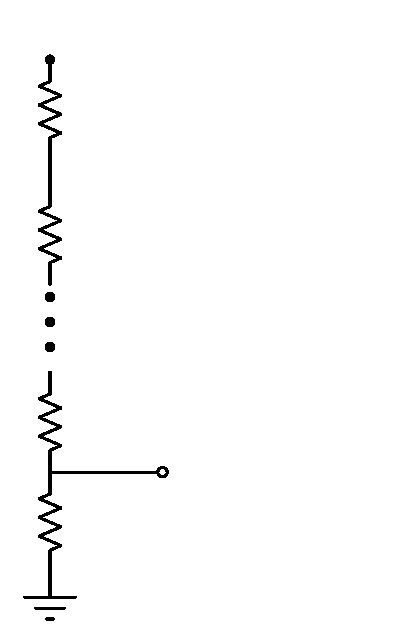
\includegraphics[scale=1]{images/Voltagedivider.eps}\\
   % translate x=208 y=444 scale 0.38
   \putbox{0.31in}{3.87in}{1.20}{$V_{applied}$}%
   \putbox{1.06in}{1.12in}{1.20}{$V_{meaured}$}%
   } % close 'parbox'
   } % close 'scalebox'
   \vspace{-\baselineskip} % this is not necessary, but looks better

			\caption{voltage divider to measure the applied
			voltage}
		\end{figure}
		
	\item Power dissipation: it could be measured 
		\begin{equation}
			P = V_{in} \times I_{in}
		\end{equation}
		where $V_{in}$ is the input voltage and $I_{in}$ is the 
		input  current

	\item Thrust/Lift: Due to lack of fine equiments the following
		method is used, we load the ionocraft with some wieght and 
		when the ionocraft reaches equilibrium the wieght of the 
		ionocraft is measured using a sensitive sacle.

	\item gap distance: since the gap distance measured in
		centemeters, it is safe to measured it using refular ruler.
		
\end{enumerate}
\subsection{Experiment Setup:}
\begin{enumerate}
	\item Setup 1:\\
	In Setup 1, we perepared Triangular ionocraft with side length
	10 cm, and aluminum foil hight of 4cm,
	with wooden skewers as support.
	The voltage applied $\approx 30KV$ (we couldn't measure it
	accurately due to loading effect,but the arc estaplished at
	around 1cm).
	Unfotnately the ionocraft didn't fly, the ionocraft was to
	heavy to take off, and the thrust was too weak.
	First, we try to increase the input voltage from 12 volts up
	to 19 volts,but unfournatly the thrust was too weak to make
	the ionocraft fly, also we couldn't measure the thust of
	due to lack of  equiments and the ionocraft is still fixed.

\begin{figure}[ht]
	\centering
	\includegraphics[scale=0.2]{Setup1}
	\caption{Setup 1 Triangular ionocraft with wooden skewers
	support}
\end{figure}

	\item Setup 2:\\
	In this setup we made the following changes, first the wooden
	skewers was replaced by plastic straws, second the the legnth
	of the support was reduced, and the Hight of the aluminum foil
	was reduced ( and unfournatly not measured), third the input
	voltage was increased to 30 volts.\\
	Unfournatly the ionocraft didn't fly, also the thrust was
	stronger(and agian not measured as the ionocraft was stand still
	).
	
	Now, we may make changes to the ciruit generating the High
	voltage its self, also we plan to make the ionocraft lighter
	and the collector smoother
	or at worst case change the structure itself.
	We should also change the measureing technique, to allow for
	measureing weak Lifts even when the ionocraft on the ground.
	\begin{figure}[ht]
		\centering
		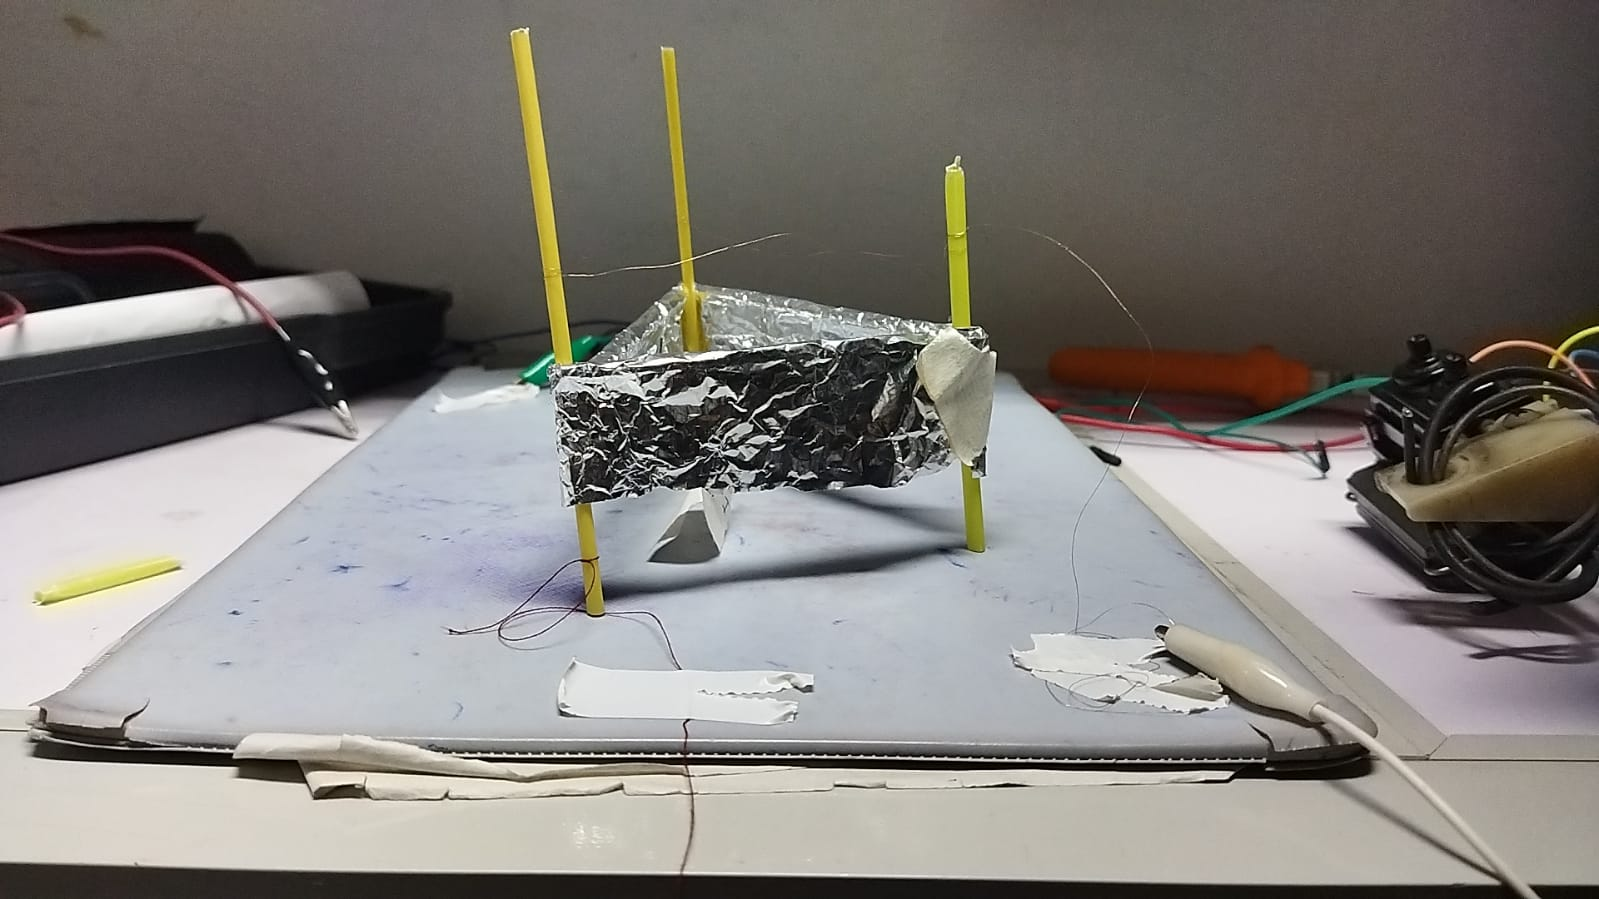
\includegraphics[scale =0.2]{setup2}
		\caption{Setup 2 Triangular ionocraft with plastic straws}
	\end{figure}

	For now we will use another Experiment data to test the models.
\end{enumerate}


\end{document}
